\chapter{Particle Physics}
\label{chap:particlephysics}

Particle physics is the study of the elementary particles and fundamental forces
of nature. By ``elementary particles'' we mean the smallest, most
basic building blocks of all structures in the universe. By
``fundamental forces'' we mean the basic kinds of interactions between
particles, from which all other possible interactions in the universe
arise.

This chapter will provide a basic introduction to the terminology
and principles of particle physics, with the goals of motivating the
research in this dissertation, and also making it understandable to
readers outside the particle physics community.

\section{The Standard Model}
\label{sec:standardmodel}

\subsection{Description}
\label{ssec:SMdescription}

The Standard Model (SM) is the scientific theory that describes
(almost) all the particles and forces we know of and their properties.
It is a relativistic quantum field theory, describing both the
behavior of particles at speeds up to (and including) the speed of
light, as well as their quantum mechanical nature.
The SM was developed over several decades of the 20\textsuperscript{th}
century through the joint efforts of theoretical and experimental physicists.
Although it is not a perfect description of all known phenomena in
particle physics, it is still widely considered to be one of the most
successful scientific theories of all time. %Citation?

The standard model describes two families of matter particles -- that is
to say, particles that give rise to tangible materials at the macro scale.
These two families are called quarks and leptons. In addition, it
describes several force-carrying particles, as well as the Higgs
boson. A sort of ``periodic table'' of these particles is given in
Figure \ref{fig:standardmodel}. A diagram showing which particles
interact with which other particles is given in Figure \ref{fig:couplings}.

\begin{figure}[h]
  \centering
  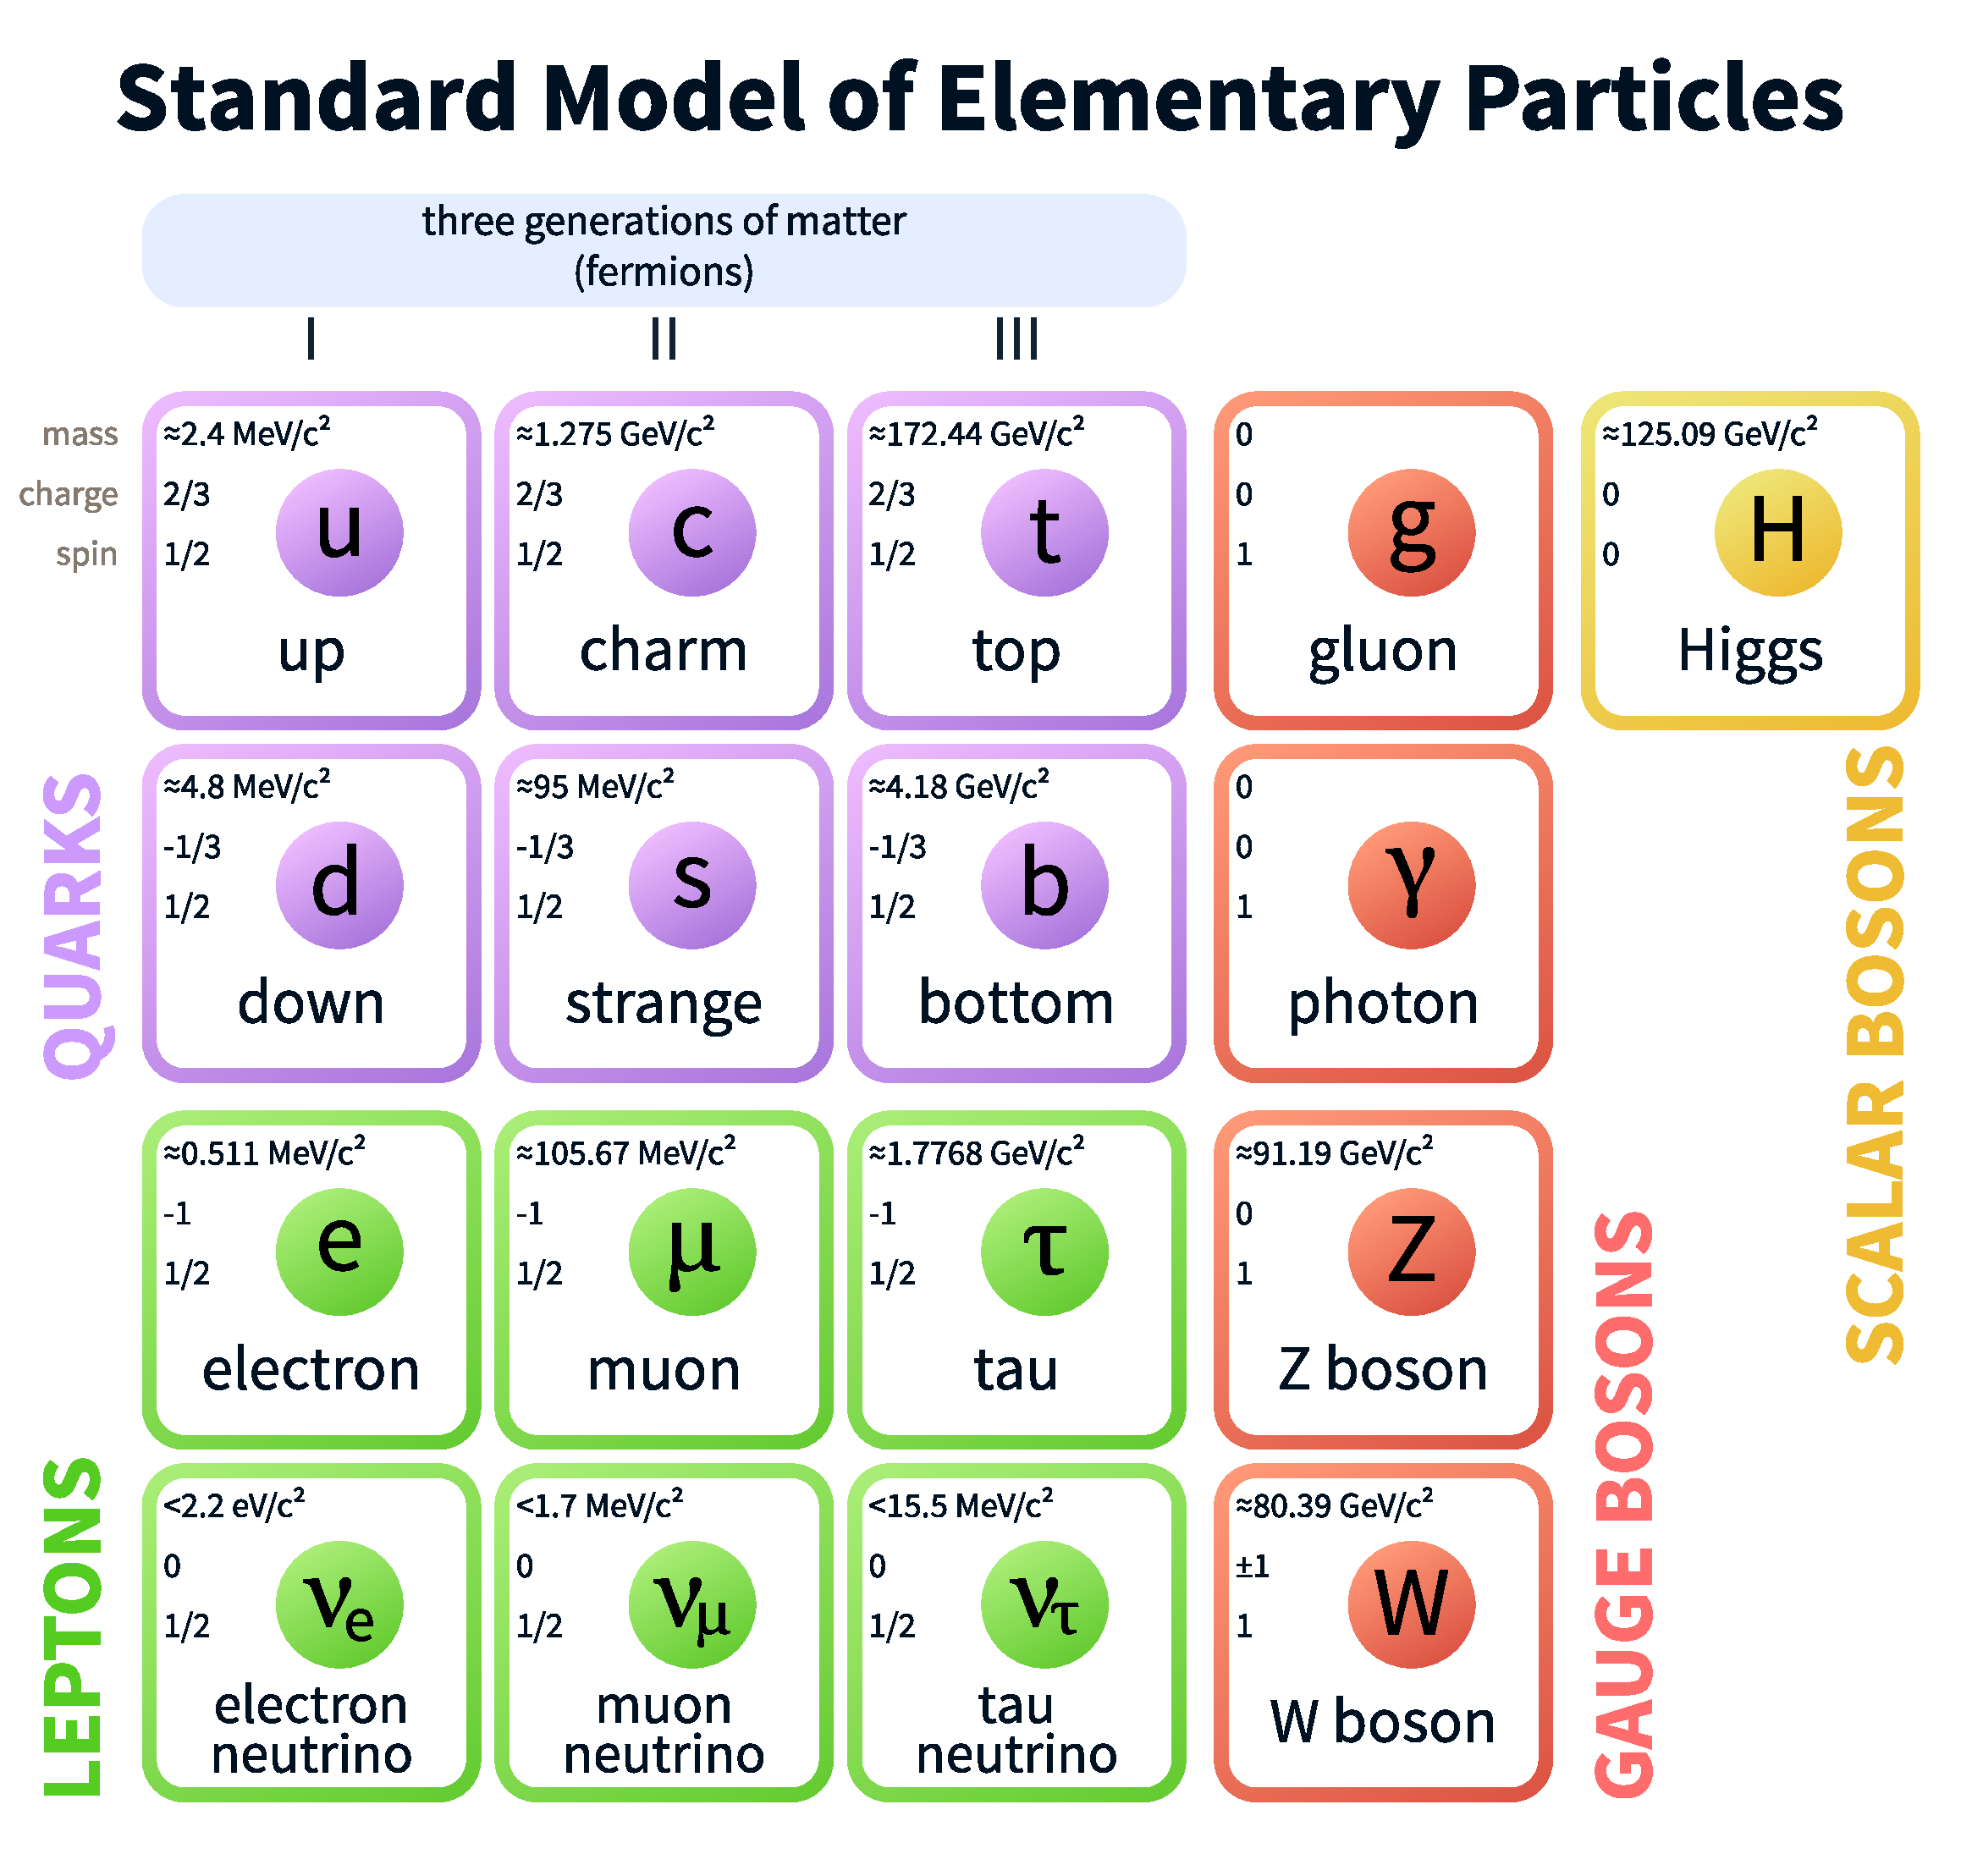
\includegraphics[width=0.75\textwidth]{figures/standard-model-light.pdf}
  \caption%[A diagram of all the particles of the standard model,
          %grouped into families of related particles.]
  {A diagram of all the particles of the standard model, grouped into
  families of related particles. Mass measurements are constantly
  being improved, and the listed mass values may not reflect the latest and
  best measurements.}
  \label{fig:standardmodel}
\end{figure}

\subsubsection*{Quarks}
There are six quarks in the SM. In order from lightest to heaviest,
these quarks are named \emph{up, down, strange, charm, bottom,} and
\emph{top}. They are often referred to using only the first letter of
their names. The up and down quarks are essential to our lives, as
they make up the nuclei of atoms: the proton is composed of two up
quarks and a down quark bound together ($uud$), and the neutron is composed of one up
quark and two down quarks ($udd$) bound together. The four heavier
quarks tend to decay into lighter quarks within a fraction of a
second, so they are generally not found in everyday matter. The up,
charm, and top quarks all have a positive charge with $\frac{2}{3}$ the
magnitude of the electron's charge, and the down, strange, and bottom
quarks have a negative charge that is $\frac{1}{3}$ that of the electron.

The top quark has several unique properties that make it important
in particle physics. Not only is
it the heaviest quark, but it is also the heaviest elementary particle
we know of, with a measured mass of approximately 173 giga-electron
volts (GeV). Compare this to approximately 2.2 mega-electron volts
(MeV) for the up quark \cite{pdg}. This mass is comparable to the mass
of an entire tungsten atom, which contains a multitude of quarks and electrons.
In addition, when the top quark decays, it has a 96\% chance of
decaying into a bottom quark and a W boson \cite{pdg}. Few other
particles have such predictable decay products. The reasons why these
properties are so important will be articulated in later chapters. % Specific reference?

\subsubsection*{Leptons}
There are three defining members of the lepton family. In order of
increasing mass, they are: the electron
($e^-$), the muon ($\mu^-$), and the tau ($\tau^-$). As their symbols
denote, these leptons each have a negative electric charge. They are
often referred to collectively as the charged leptons.
The electron is well known as the part of an atom responsible for the
majority of its chemical interactions with other atoms. Muons and taus
tend to decay within a fraction of a second, so they also tend not to
be found in everyday matter. However, they are often produced in
Earth's upper atmostphere due to bombardment of the atmosphere by
cosmic rays, originating in outer space.

For each charged lepton, there is a corresponding particle known as a
neutrino. They are known as the electron neutrino ($\nu_e$), the muon
neutrino ($\nu_{\mu}$), and the tau neutrino ($\nu_{\tau}$). As their
name suggests, neutrinos are electrically neutral - they have no
charge. In addition, neutrinos have extremely small masses. In fact,
the SM considers them to be massless particles, but experimental
results show they have non-zero masses of less than one electron volt
(eV) \cite{pdg}. Neutrinos also have an extremely small probability of
interacting with matter. In practice, this makes neutrinos
difficult or impossible to detect. The experimental implications of
this fact will be described in chapter \ref{chap:hardware}.

\begin{figure}[h]
  \centering
  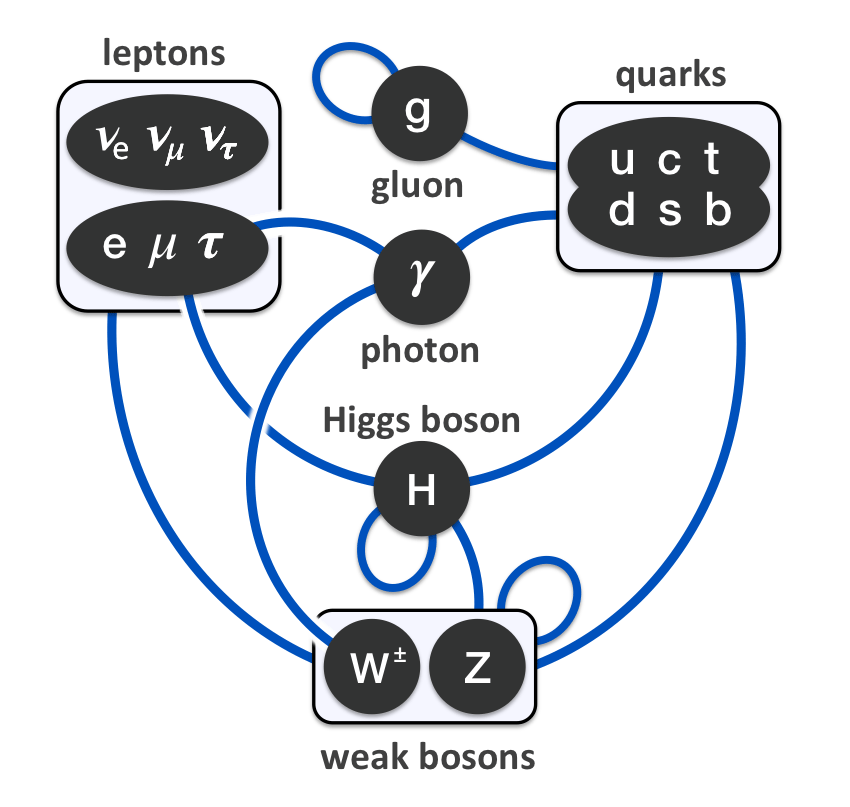
\includegraphics[width=0.75\textwidth]{figures/couplings.png}
  \caption{A diagram of the interactions, or couplings,
    between the particles of the standard model. Particles or groups
    of particles connected by blue lines are able to interact with
    each other.}
  \label{fig:couplings}
\end{figure}

\subsubsection*{Force Carriers}
The standard model describes four force-carrying particles. These
particles are the physical manifestations, or \emph{quanta}, of the forces
they convey. In general, matter particles interact with other matter
particles through the force-carriers. However, not all particles are
able to interact with all forces.

The photon ($\gamma$) is the quantum of the electromagnetic
force. Thus every time two particles interact electrically or
magnetically, they do so by exchanging photons. Only particles that
have a non-zero electric charge can interact electromagnetically. Thus
we say the photon \emph{couples to} charged particles. All quarks, as
well as the charged lepton, carry electric charge. In addition, the
photon is the particle of light. Thus when an object is illuminated by
light, it is actually being bombarded by photons. The photon travels
at the speed of light, which is only possible for particles that have
zero mass.

The gluon ($g$) is the carrier of the strong nuclear force. The strong
force is responsible for binding together quarks to form protons,
neutrons, and other composite particles (known collectively as
\emph{hadrons}). This same interaction also causes protons and neutrons to
bind together and form atomic nuclei. Gluons couple to any particle
that has so-called \emph{color charge}, namely quarks and
other gluons. Although gluons are in principle massless, the energy of
their collective interactions actually makes up more than 99\% of the
mass of protons and neutrons.

The W and Z bosons ($W^+$, $W^-$, $Z$) carry the weak nuclear force. This
force is best known for mediating radioactive $\beta$-decay through
the W-bosons. In addition, the only way quarks can change flavor is by
interacting via a W-boson, so W-bosons are very commonly produced when
heavier quarks decay into lighter ones.
Particle physicists know the Z-boson best for its
role in the Drell-Yan process, where pairs of quarks convert into
pairs of charged leptons. The W and Z bosons couple to all matter
particles. In addition, they are capable of coupling to each other,
though such interactions are rare. The W bosons have a mass of around
80 GeV, and the Z boson has a mass around 91 GeV \cite{pdg}.

\subsubsection*{Higgs Boson}
The Higgs boson is included here for completeness, and for the benefit
of the curious reader, although it plays at best a minimal
role in the research described in this dissertation. The Higgs
boson is neither a force-carrying particle nor a matter particle, but
something else entirely. It is the manifestation, or quantum, of the
Higgs field, a field that permeates the entire universe, and endows
mass upon most elementary particles. The top quark is so massive
because it couples very strongly to the Higgs field. Similarly, the
photon is massless because it does not couple to the Higgs field at all.
The Higgs boson itself was discovered to have a mass of about 125 GeV,
which means the Higgs must couple to itself.

\subsubsection*{Spin}
All particles (both elementary and composite) have
a property known as spin. Spin is an intrinsic property, just like
mass or electric charge. But unlike those properties, spin is quantum
mechanical in nature. So a particle's spin is sometimes called its
spin quantum number. All particles can be divided into two categories
based on their spin quantum numbers: particles whose spin is an
integer (0, 1, 2, 3...) are called \emph{bosons}, and particles whose
spin is a half-integer ($\frac{1}{2}, \frac{3}{2}, \frac{5}{2}...$)
are called \emph{fermions}. Figure \ref{fig:standardmodel} already
labels which particles are fermions and which are bosons, but even
absent those labels, you could see that quarks and leptons are all
fermions because they have spins of $\frac{1}{2}$, and the force
carriers and the Higgs particle are all bosons.

\subsubsection*{Antimatter}
For every matter particle, there also exists a corresponding
antiparticle. These are collectively referred to as
antimatter. Antiparticles generally have the exact same properties as
their normal-matter partner, except that their electrical charge (if
they have one) is opposite in sign. Thus the anti-electron (also
called a positron) has a positive electrical charge instead of
negative. The antimatter versions of the charged leptons are indicated
with a plus in their symbol ($e^+, \mu^+, \tau^+$), and all other
antiparticles have a bar on top of their symbol ($\bar{u},
\bar{b}, \bar{\nu_{\mu}}$, etc.). When a particle meets its own
antiparticle, they usually produce high-energy photons, or sometimes
Z-bosons. Because antimatter
annihilates on contact with normal matter, it is not found
in large quantities in our universe. However, very small quantities can be
produced by energetic particle collisions in nature, and in manmade
particle colliders.

%%%%%%%%%%%%%%%%%%%%%%%%%%%%%%%%%%%%%%%%
% Do I need to explain Feynman diagrams?
%%%%%%%%%%%%%%%%%%%%%%%%%%%%%%%%%%%%%%%%

\subsection{Successes}
\label{ssec:SMsuccesses}

The predictions of the standard model have been borne out in a
staggering number of experiments over the last several decades. This
unprecedented success has led the standard model to be labeled as one
of the most successful scientific theories ever formulated. % Probably need a reference for this.
-Give some statistics on number of published particle physics papers
-How many of them substantiate the predictions of the SM?
-Give some examples of remarkable successes (e.g. the Higgs discovery)

\subsection{Shortcomings}
\label{ssec:SMshortcomings}

Despite the standard model's vast successes, it is not a complete
theory of all particles and interactions in the universe. Physicists
have observed a number of phenomena that are not described within the
framework of the standard model. Additionally, the information needed to
build a universe cannot all be predicted from the standard model
alone. Some of these shortcomings are presented here.

\subsubsection*{Gravity and the Hierarchy Problem}
When describing the fundamental forces of nature in Section
\ref{ssec:SMdescription}, one force was conspicuous by its absence:
gravity. Although gravity is the most apparent force of nature in our
everyday lives, and was the first to be described mathematically,
the standard model is still unable to incorporate the workings of
gravity. Einstein's general theory of relativity does a marvelous job
describing gravity on the scale of large objects, such as stars or
galaxies. However, physicists have so far been unable to formulate a
theory of gravity consistent with quantum mechanics, a necessary step
to incorporate gravity into the standard model.

One key stumbling block in the quest to quantize gravity (though by no
means the only one) is called the Hierarchy Problem. In plain language, the
problem is that gravity is weaker than the other fundamental forces by
a staggering 20 to 30 orders of magnitude, depending on the distance
scale considered. Any attempt to unite gravity and the other forces
of nature must find a way to bridge this gulf.

\subsubsection*{Fine Tuning}
Another perceived deficit of the standard model is the fact that many
of the fundamental constants of nature are not part of the theory. For
example, the standard model correctly predicts the existence of the six
flavors of quarks, but it does not predict what their masses will be;
the masses must be measured experimentally. Similarly, the Standard
Model offers no clue to the strength of the various forces of nature,
only their existence. In total, the standard model has 19 independent
parameters that cannot be derived from other information in the
theory. Some theorists object to this large number as being inelegant
and unwieldy, feeling that a fundamental description of the universe
should have fewer free parameters.

\subsubsection*{Dark Matter}
Physicists and astronomers have been observing the motions of stars
for longer than recorded history. Starting in the late 19\textsuperscript{th}
century, physicists tried to calculate the mass of the Milky Way
galaxy based on the stars they could see through their
telescopes. They soon discovered that the galactic mass estimated from
visible stars was significantly less than the galactic mass
estimated from the rate at which those stars rotate about the
galactic center. In the first half of the 20\textsuperscript{th}
century, scientists noticed the same discrepancy for other galaxies
as well. They hypothesized that galaxies also contained some kind of
matter that was not visible through telescopes (hence \emph{dark}),
but that nevertheless exerted a gravitational pull. In fact, we now
estimate that only about $\frac{1}{6}$ of the mass of the universe consists
of visible matter such as stars and planets. % Citation needed

Since all matter is made of particles, the particle physics community
has also taken a strong interest in the problem of this unknown
substance. Careful astronomical observations and detailed calculations
have shown that dark matter does not interact with the strong or
electromagnetic forces. % Citation needed
However, it is believed to participate in the weak interaction. % Why? Also, citation needed!
Further work has shown that no standard model particle (or composite
of standard model particles) can have these properties and be
consistent with astronomical observations of temperature and % Ick, I hate how this is phrased. Rewrite!
density. Therefore, the existence of dark matter seems to require
physics beyond the standard model (BSM).

\subsubsection*{Dark Energy}
Observations of the cosmic microwave background (CMB) and of the % When? By whom?
doppler shifts of various stars have demonstrated that the universe is
expanding at an accelerating rate. This result surprised many
scientists, becase in principle the inexorable pull of gravity should
cause the universe to collapse in on itself eventually. Yet something
is driving an outward push that is speeding up instead of slowing
down. Scientists use the term ``dark energy'' to refer to the unknown
and unobserved energy driving this expansion.
% Does this really necessatate an extension of the SM?
% May be easier to delete this part entirely.

\subsubsection*{Neutrino Masses and Oscillations}
The standard model predicts that neutrinos should be entirely
massless. And for many years, observations of processes that produced
neutrinos, such as $\beta$-decay, seemed to confirm this
supposition. However, in 19XX, observations of neutrinos produced in % Year!
the sun showed that the rate of electron neutrinos reaching the earth
was only a third of what was expected. Further experiments eventually
showed that neutrinos actually change back and forth between their three % Citation for neutrino oscillations?
flavors as they travel through space. This change made it impossible
for neutrinos to be massless, because massless particles must travel
at the speed of light, and therefore do not experience the passage of
time. But since neutrinos morph between different states, clearly they
must have some experience of time passing. These neutrino
oscillations require an extension of the standard model in order to
explain how the neutrinos acquire mass, and how they are able to
change identities in defiance of the principles of particle physics.

\section{Supersymmetry}
\label{sec:susy}

Physicists have proposed a number of theories to explain the various
shortcomings of the standard model. One particular class of theories,
known as supersymmetry (or SUSY for short), is extremely popular for
the elegant ways it can fill a number of these gaps. Although there
are numerous variations of supersymmetric theories, they all have one
defining feature in common. For every standard model particle, SUSY
postulates the existence of another particle with mostly the same
properties, but with a spin that differs by $\frac{1}{2}$. Thus every standard model
fermion would have a corresponding ``superpartner'' that is a boson,
and every standard model boson would have a superpartner that is a
fermion \cite{susyprimer}.

\subsection{Sparticles}
\label{ssec:susysparticles}

Supersymmetry uses a unique, sometimes quirky nomenclature to refer to
the new particles it postulates. The partners of standard model
fermions are named by prefixing the existing name with an `s'. Thus
the two families become \emph{squarks} and \emph{sleptons}, and the
individual members of those families are named, e.g., \emph{sup,
  sbottom, selectron, sneutrino}, etc. Meanwhile the partners of
standard model bosons gain the suffix \emph{-ino}, which replaces the
suffix \emph{-on} if present. Thus we arrive at the names
\emph{gluino, photino, Zino, Wino}, and \emph{Higgsino}. The symbols
for these particles are generally formed by adding a tilde on top of
the original particle's symbol, so that a scharm squark is notated
$\tilde{c}$, a gluino is notated $\tilde{g}$, etc.

These superpartners are capable of mixing with each other to form
different particles, which may not correspond exactly to standard
model particles. Of particular note are the neutralinos
($\lsp_1, \lsp_2, \lsp_3, \lsp_4$), made by mixing the photino, zino,
and Higgsino; and the charginos ($\chargino_1, \chargino_2$), made by
mixing charged Winos and charged Higgsinos.

It is worth noting that if SUSY were a perfect symmetry, all
sparticles would have the same masses as their corresponding
particles. However, to date, no sparticles have been
observed, implying that most sparticles (if they exist) must be too
heavy to produce using our current particle colliders. Since the
equality of masses is destroyed, we say SUSY is a \emph{broken
  symmetry} \cite{susyprimer}.

\subsection{Rationale}
\label{ssec:susyrationale}

One of the features that makes SUSY very attractive is its ability to
solve the hierarchy problem. The exact nature of this solution
invokes quantum field theory, and is not terribly pertinent to the
research described in this dissertation. However, the essence is
that the massive standard model particles should make the Higgs mass
squared ($m_H^2$) blow up to an enormous number; by introducing a
new boson for every SM fermion, and vice-versa, SUSY cancels out
the effects of the SM particles, and allows $m_H^2$ to take on a
more reasonable value \cite{susyprimer}.

In addition, SUSY provides particles that may be good candidates to
explain dark matter. At the moment, the most popular explanation for
the composition of dark matter is weakly-interacting massive particles
(WIMPs). These are particles that primarily interact through the weak
force, and that also have mass, allowing them to exert a gravitational
pull. The neutralinos fit this bill nicely. In addition, the dark
matter particle must be stable. The lightest supersymmetric particle
(LSP) is expected to be stable due to conservation laws associated
with supersymmetry, and many SUSY models predict that the lightest
neutralino, $\lsp_1$, actually \emph{is} the LSP. Thus the lightest
neutralino makes a tantalizing dark matter candidate
\cite{susyprimer}. We will assume moving forward that $\lsp_1$ is the
LSP, and will use the two terms interchangeably.
% Need citation for this stuff?

